\documentclass[12pt,a4paper]{report}

\usepackage[utf8]{inputenc}
\usepackage[english]{babel}
\usepackage[left=2.5cm,right=2.5cm]{geometry}

\usepackage{amsmath}
\usepackage{blindtext}
\usepackage{amsfonts}
\usepackage{amssymb}
\usepackage{graphicx}
\usepackage{multicol}
\usepackage{fancyhdr}
\usepackage{wrapfig}
\usepackage{lipsum}
\usepackage{caption}
\usepackage[square,numbers]{natbib}
\usepackage[pagebackref]{hyperref}

\author{S. Bourgeois}


\begin{document}

%\bibliographystyle{plainnat}
\bibliographystyle{abbrvnat}
%\setcitestyle{number,open={a},close={a]}} %Citation-related commands
\setcitestyle{author,numbers}

\pagestyle{fancy}

\fancyhead{} % clear all header fields
\fancyhead[L]{\small Nuclear energy for space exploration: A technological necessity \\ or a risky gamble for humanity and the wider environment ?}
\fancyhead[R]{\small BOURGEOIS Sacha\\
2025}
\fancyfoot{} % clear all footer fields
\fancyfoot[C]{\thepage}

\begin{titlepage}
\begin{center}

\textup{\small {\bf First year of Master's Internship} \\ Report}\\[2cm]

% Title
\LARGE \textbf {Nuclear energy for space exploration: \\
A technological necessity or a risky gamble for humanity and the wider environment ?}\\[3cm]



       

% Submitted by
\normalsize Submitted by \\[0.2cm]
\textbf{S. Bourgeois}\\
M1 PFA\\
\vspace{0.5cm}
Under the guidance of\\[0.2cm]
\textbf{S. Porteboeuf-Houssais, J. Donini}\\
Profs.



\vspace{1cm}

% Bottom of the page

\includegraphics[width=0.2\textwidth]{img/UCA-logo.png}\\[0.5cm]
\Large{Department of Physics}\\
\normalsize
\textsc{Université Clermont Auvergne}\\
4 Avenue Blaise Pascal\\
63178 Aubière\\
\vspace{0.2cm}
11th of June 2025

\end{center}

\end{titlepage}
\newpage

\chapter*{Acknowledgment}
\quad Before further development on this work I would like to thank those who have helped to structure and carry it out.\\

First and foremost I would like to thank my tutors Mister Donini and Miss Porteboeuf-Houssais for their involvement and their guidance during this project and this first year of Master's. \\

Then comes the rest of our team, Victor Auga-Bascou, Yael Chahinian and Yvon Marthon with whom I have worked for these pasts eight weeks. I want to thank them for their patience and their teamwork abilities.\\

I also thank Pauline D., Pauline P., Camille D. and Elisa B for proofreading this report, for their hospitality and their unwavering support. \\

Lastly, I thank you, reader of this report, for taking some of your time to understand and grade this work. Without you all of this would be useless.
\newpage
\chapter*{Foreword}

Let us first understand what this work constitutes and how it was structured.\\


For the past two months Victor, Yael, Yvon and I have studied, under the tutoring of Sarah and Julien.
This work we have been doing differs from a "classical" internship in that it was mostly bibliographic until the end whence it differed widely. \\

Indeed, we had a mock-up debate wherein each of us students had to take on different roles and perspectives while trying to answer our research question : "Nuclear energy for space exploration: A technological necessity or a risky gamble for humanity and the wider environment ?".\\
This TER used to be a class centered around "Nuclear energy and Society", taught during the second semester of master's, its objective was to spur students into developing  their ability to communicate and debate around a science-focused subject as well as to lead bibliographic research.\\

Our work differs from those that came before us in that we didn't focus our research on nuclear power plants or atomic weapon proliferation but rather on space exploration and radiation shielding.\\

We hope that you will find this report interesting and perhaps even learn a thing or two along the way.
\newpage

\tableofcontents


\chapter*{Introduction}

% 	states your hypothesis 	explains how you derived that hypothesis and how it connects to previous research; gives the purpose of the experiment/study

\quad Space exploration and technologies have long been open fields of active research and in that, interplanetary travel and planetary exploration are of major interest for agencies, companies and amateurs alike such as NASA, ESA, Space X or Copenhagen Suborbital.\\


In this report we will study the following question : \\
"Nuclear energy for space exploration: A technological necessity or a risky gamble for humanity and the wider environment ?".\\

For that purpose we will study the research on Nuclear Termal Rockets
We will assume the role of Elon Musk, CEO of Space X a space technology company whose objective it will be to send a team of astronauts to the planet Mars and whose questionable ethics will lead us at the limit of what is considered acceptable in terms of radiation exposure, in opposition to NASA moto "as safe as possible" we would follow Elon's "move fast, break things".\\
For this purpose we will study nuclear propulsion to show it is superior to classical means of propulsion for a trip to Mars, as well as composite material radiation shielding and why it would be necessary for such a mission.\\

We will show that, assuming today's technology, it is quite unrealistic to propel a crew of four to Mars and back using anything else than a NTR and will try to show how nuclear energy and fissile materials can be used quite safely in the context of space propulsion. We will also show how much weight can be saved on shielding while still keeping the astronauts alive and healthy for the duration of the flight.

This report is heavily based on the book by \citet{hoffman1997} at Johnson Space Center, a volume that is dedicated to planning, in great details a manned mission to our neighbor Mars.

\addcontentsline{toc}{chapter}{Introduction}

\chapter{Methods}
%details how you tested your hypothesis clarifies why you performed your study in that particular way

\section{Nuclear Propulsion}
\subsection{Specific Impulse}
Specific impulse is a measure of how efficiently a reaction mass engine generates thrust.\\
It can be derived from the rocket thrust equation given by :
\begin{equation}
F = \dot{m}v_e + (p_e - p_0)A_e 
\end{equation}
Where $p_e$ and $p_0$ are respectively the pressure of the exhaust and of the atmosphere, $v_e$ is the speed of the exhaust, $A_e$ is the area of the exhaust, $\dot{m}$ is the mass flow rate and $F$ is the thrust.\\
From which can be defined the equivalent velocity expressed by:
$$V_{eq}=v_e+\frac{(p_e-p_0)A_e}{\dot{m}}$$
As well as the total impulse:
$$I=F\Delta t = \int F dt = \int \dot{m}v_{e}dt=mv_{e}$$
Which allows us to finally define the specific impulse as:
\begin{equation}
I_{sp}=\frac{I}{mg_0}=\frac{v_{e}}{g_0}=\frac{F}{\dot{m}g_0}
\end{equation}
Where $g_0$ is the gravity acceleration at sea level.
\newpage
\subsection{Rocket Equation}

The Tsiolkovsky rocket equation also known as the ideal rocket equation defined as follows: 
\begin{equation}
\Delta v=v_e\ln\left(\frac{m_0}{m_f}\right)=I_{sp}g_0\ln\left(\frac{m_p}{m_f}+1\right)
\end{equation}
Where $m_0$ the initial mass of the rocket, also known as wet mass, $m_f$ the final mass, or dry mass, of the rocket, and $m_p$ the mass of the propellant.
Given an effective exhaust velocity this equation allows us to find how much propellant mass is needed for a given change in velocity.
\subsection{$\Delta v$ Budget}
The concept of $\Delta v$ budget is an estimate of the total change of velocity required to perform each propulsive maneuver over the duration of a given mission this quantity can then be used as described in 1.1.2.\\
\begin{figure}[hbtp]
\centering
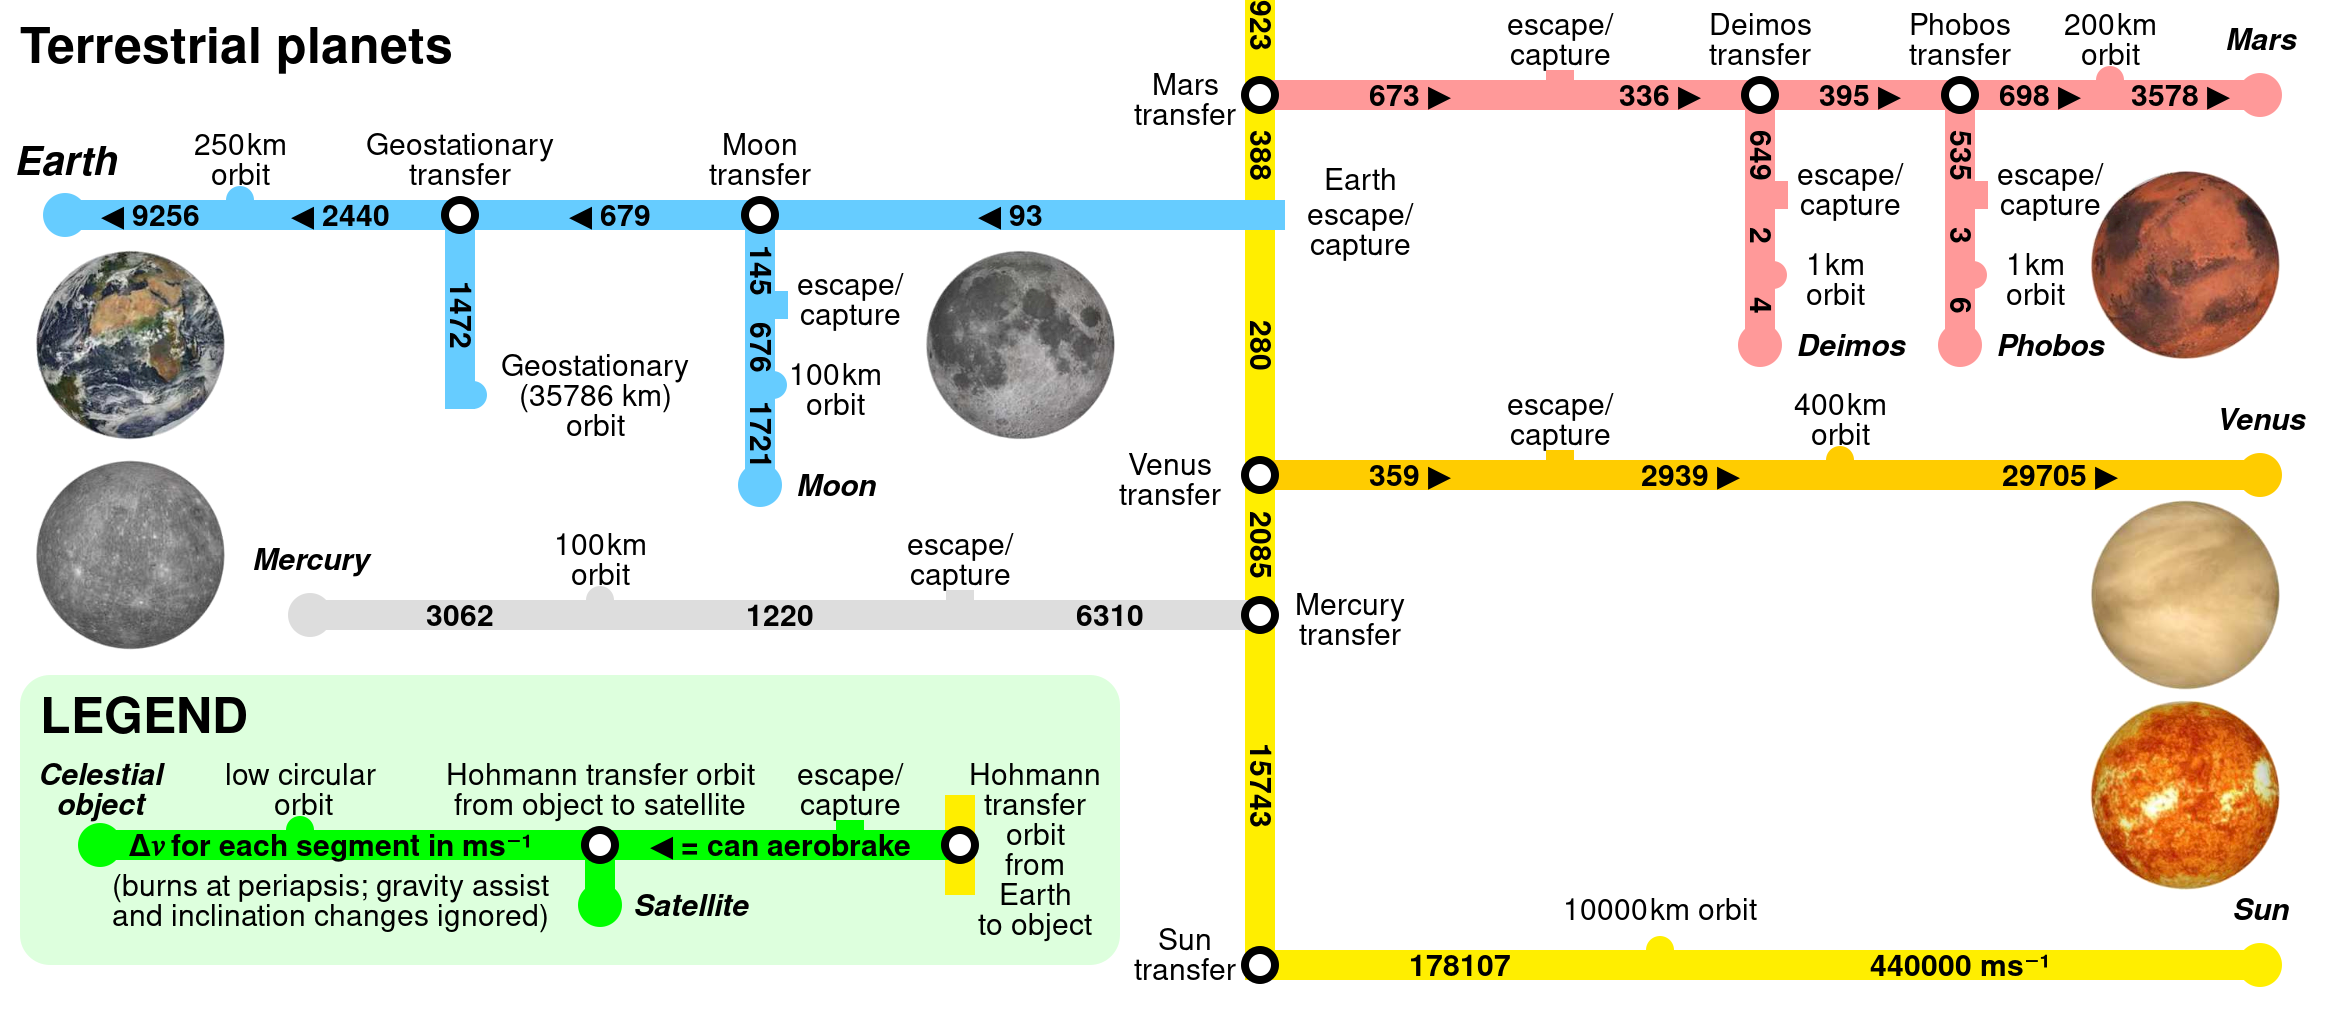
\includegraphics[scale=.2]{img/dv.png}
\caption{Delta-v map, assuming burns at periapsis, gravity assist, and ignoring inclination changes}
\end{figure}

For an Earth-Mars trip, a conservative estimate is located around $18000m.s^{-1}$, it is important to note that even though one could save up on fuel by using more efficient transfer techniques this would also come at the expanse of travel time, which, it will be shown in later sections, becomes a major hurdle of space travel. On the other hand aerobreaking is an option both on Earth and Mars and should be fully utilized to save up on fuel.
\newpage
\subsection{NTR}
\citet{finseth1991} descries solid core nuclear thermal rockets, such as the NERVA-XE as making use of highly enriched U-235 fission reactor through which liquid hydrogen is passed serving as both coolant and propellant as well as an additional, good quality radiation shield.
\begin{figure}[hbtp]
\centering
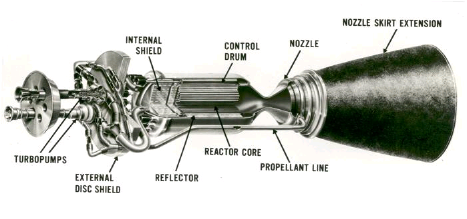
\includegraphics[scale=.7]{img/NERVA-solid-core-nuclear-propulsion-system.png}
\caption{NERVA solid core nuclear propulsion system. Source:
NASA.}
\end{figure}




\newpage

\section{Radiations in Space}


\subsection{Shielding}
Astronauts are exposed to higher doses of radiation in interplanetary space mainly due to the lack of a magnetosphere and an atmosphere shielding them from SEP and GCR, the two main types of radiations they would be exposed to for an inter-planetary journey such as one from Earth to Mars. \\
The dose grows stronger as one gets further away from the Earth as its magnetosphere grows weaker and its atmosphere thinner the further away one gets from it.
As for Mars, who lacks a strong magnetosphere such as Earth's, it does have a CO2 atmosphere which shields it from space born radiations, though less than Earth's thicker atmosphere.\\
\citet{baumstark2002life} \citet{cucinotta2009} show that the unprotected human body is quite vulnerable to radiation, long term exposure and accumulation of radiations. All can lead to sever health effects.\\

Although the legislation is lacking for space the IAEA, the UN legislative body, specifies a dose of $20mSv$ per year averaged over five consecutive years (100 mSv in 5 years) and of $50mSv$ in any single year for occupational workers as expressed in \citet{IAEA-GSG}. A quantity well under was is proposed in the study from \citet{hoffman1997} as can be observed in figure 1.4. 

\begin{figure}[hbtp]
\centering
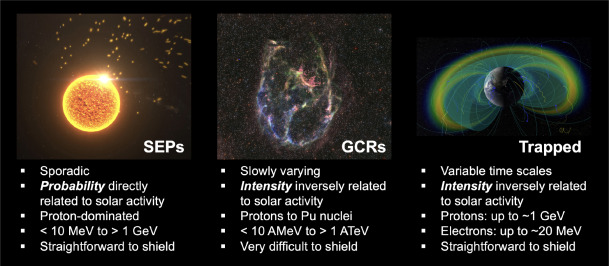
\includegraphics[scale=1]{img/Major characteristics of SEPs GCRs and trapped particle radiation.jpg}
\caption{Major characteristics of SEPs, GCRs, and trapped particle radiation. Images courtesy of NASA Scientific Visualization Studio. SEP image credit: NASA’s Goddard Space
Flight Center Conceptual Image Lab, GCR image credit: NASA/STScI/CXC/SAO, processing by Judy Schmidt, CC BY-NC-SA, Trapped image credit: NASA’s Scientific Visualization
Studio.}
\end{figure}

\newpage

The relativistic version of the Bethe–Bloch formula for the mean energy loss (stopping power) for a fast charged particle traveling through a material as described in  \citet{groom2000passage} is expressed as follows:
\begin{equation}
- \left\langle \frac{dE}{dx} \right\rangle = \frac{4\pi}{m_e c^2} \cdot \frac{n z^2}{\beta^2} \cdot \left(\frac{e^2}{4\pi \epsilon_0}\right)^2 \left[ \ln\left( \frac{2 m_e c^2 \beta^2}{I\cdot (1-\beta^2)} \right) - \beta^2 \right]
\end{equation}

Where: \\
\begin{minipage}[b]{0.5\linewidth}
\vspace{0.5cm}
- $m_e$ the electron resting mass\\
- $c$ the speed of light in vacuum\\
- $e$ the electron charge\\
- $\epsilon_0$ the vacuum permittivity\\
- $\beta=\frac{v}{c}$\\
- $n=\frac{N_a\cdot Z \cdot \rho}{A\cdot M_u}$\\
\end{minipage}
\begin{minipage}[b]{0.5\linewidth}
- $z$ charge of the studies particle\\
- $v$ speed of the particle\\
- $-E$ the energy lost by the particle\\
- $x$ over the distance\\
- $n$ target electron number density \\
- $I$ target mean excitation energy \\
\end{minipage}


This report will make use of NIST's tool, PSTAR \citet{STAR}.
\\
With a default option, PSTAR generate the stopping powers and ranges for protons tabulated in ICRU Report 49 \citet{deasy1994icru} for 74 materials at a standard grid of 133 kinetic energies between 1 keV and 10 GeV for protons.



\vspace{2cm}

\begin{minipage}[b]{0.5\linewidth}
\centering
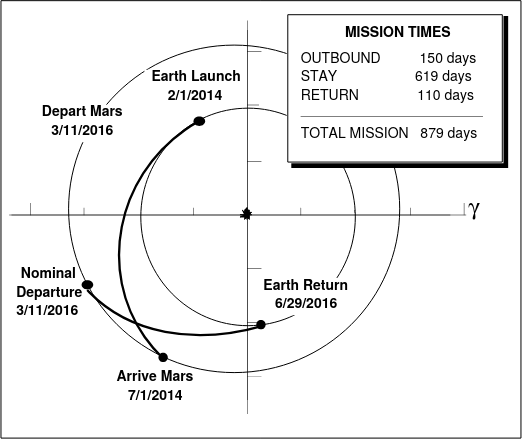
\includegraphics[width=1\textwidth]{img/optimised traj.png}
\captionof{figure}{2014 fast-transit window courtesy of the book from \citet{hoffman1997}}
\end{minipage} 
\hfill
\begin{minipage}[b]{0.35\linewidth}
In space, astronauts are exposed to three main kind of radiation environments, SEP, GCR and trapped radiations. The purpose of this report will mainly focus on SEP and GCR radiations as the time spent around the Earth and in the Van-Allen belt will be insignificant compared to the whole duration of the mission as highlighted in figure 4.1.
\end{minipage}



\newpage
\begin{minipage}[b]{0.35\linewidth}
\subsection{SEPs}
SEP are high energy charged particles originating in the solar atmosphere and transported by solar winds. They are mostly composed of high energy protons as reported in \citet{jiggens2019}. Figure 1.5 shows the energy spectra from the 1989 solar event that resulted in a complete blackout of Hydro-Québec's power grid.
\end{minipage}
\hfill
\begin{minipage}[b]{0.5\linewidth}
\centering
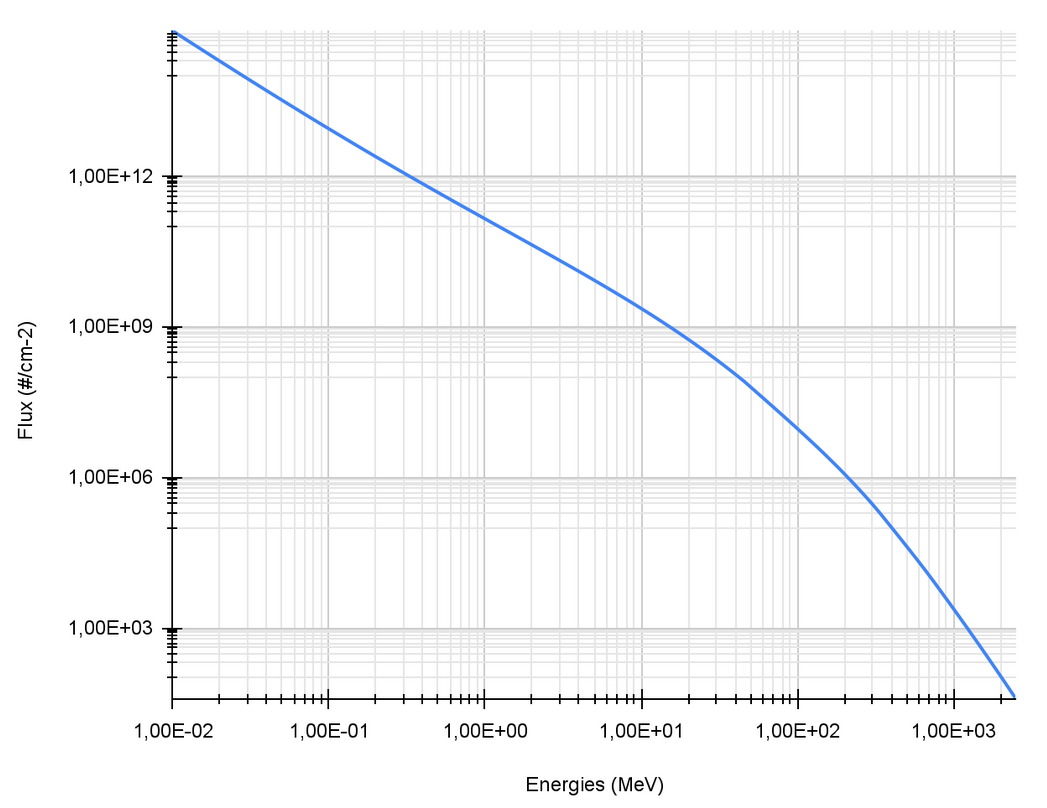
\includegraphics[width=1\textwidth]{img/proton flux 1989.png}
\captionof{figure}{The energy spectrum of the 9-13th of march 1989 solar storm}
\end{minipage} \\
\hfill\\



\begin{minipage}[b]{0.5\linewidth}
\centering
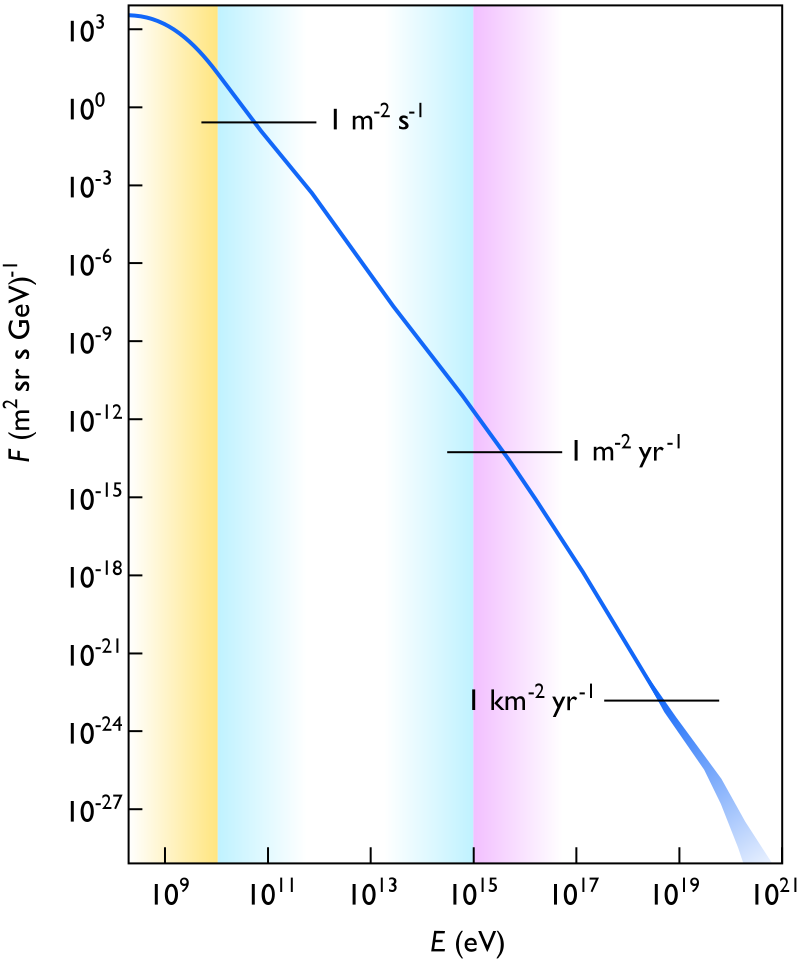
\includegraphics[width=1\textwidth]{img/Cosmic_ray_flux_versus_particle_energy.svg.png}
\captionof{figure}{Cosmic Flux Versus Particle Energy At The Top Of Earth's Atmosphere \citet{sharma2008}}
\end{minipage}
\hfill
\begin{minipage}[b]{0.35\linewidth}
\subsection{GCRs}
CGR are high energy particles mostly composed of protons and HZE ions, some of them come from our sun but from our galaxy and other galaxies as well. The bulk of the flux is deflected to space by the heliosphere. Therefore, the solar cycle and thus the strength of the sun's magnetic sphere has a major influence on the influx of GCRs.
Solar maximums and minimums, the time where the sun's activity is respectively at its maximum and its minimum will play a major role on how GCRs are dealt with.
\end{minipage}

\newpage

\subsection{Dosimetry}

\subsubsection{Absorbed Dose}

Absorbed dose is a dose quantity which represents the specific energy (energy per unit mass) deposited by ionizing radiation in living matter.

\begin{equation}
\bar{D_T}=\frac{\int_TD(x,y,z)\rho(x,y,z)dV}{\int_T\rho(x,y,z)dV} \quad (Gy)
\end{equation}

Where:
\\
- $\bar{D_T}$ is the mass-averaged absorbed dose of the entire item $T$\\
- $T$ is the item of interest\\
- $D$ is the absorbed dose density (absorbed dose per unit volume) as a function of location\\
- $\rho(x,y,z)$ is the density (mass per unit volume) as a function of location\\
- $V$ is volume



\subsubsection{Equivalent Dose}

\quad Equivalent dose is a dose quantity representing the stochastic health effects of low levels of ionizing radiation on the human body which represents the probability of radiation-induced cancer and genetic damage.

\begin{equation}
H_{T}=\sum _{R}W_{R}\cdot D_{T,R} \quad (Sv)
\end{equation}

Where:\\
- $W_R$ is the radiation weighting factor defined by regulation \citet{valentin20072007}. See Figure 4.3 for the values of $W_R$.


\subsubsection{Effective Dose}

\quad Effective dose is a dose quantity in the International Commission on Radiological Protection (ICRP) system of radiological protection. It is a good measure of the health risks associated with radiations as highlighted in \citet{protection2007icrp}.

\begin{equation}
E=\sum _{T}W_{T}\cdot H_{T}=\sum _{T}W_{T}\sum _{R}W_{R}\cdot {\frac {\displaystyle \int _{T}D_{R}(x,y,z)\rho (x,y,z)dV}{\displaystyle \int _{T}\rho (x,y,z)dV}}
\end{equation}

Where:\\
- $W_{R}$ is the radiation weighting factor defined by regulation. See Figure 4.4.\\

Figure 4.7 can be used as a visual guide for the different calculations processes.

\newpage

\chapter{Results}
%provides raw (i.e., uninterpreted) data collected (perhaps) expresses the data in table form, as an easy-to-read figure, or as percentages/ratios

\section{Propulsion}
\subsection{Nuclear Propulsion}
Here has been compared the difference in the fuel to dry mass ratio when using different technologies using Eq 1.3 and taking a $\Delta v$ of 5543 m.s-1, accounting for the use of the nuclear engine as the transfer engine, ie. the rocket would be sent to space and would land using chemical engines and the NTR would only be fired from LEO to LMO.

\vspace{.5cm}

\begin{minipage}[b]{0.49\linewidth}
\centering
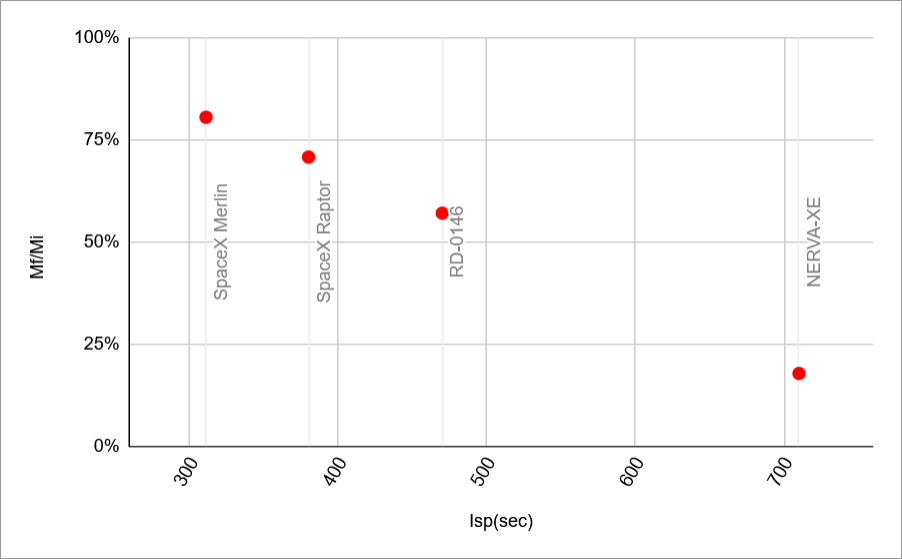
\includegraphics[width=1\textwidth]{img/ratio.png}
\captionof{figure}{Ratio of fuel to dry mass relative to Isp for a typical Earth-Mars mission}
\end{minipage} 
\hfill
\begin{minipage}[b]{0.45\linewidth}
Liquid hydrogen is a propellant of choice due to its low molecular weight, which allows for high $I_{sp}$ as well as its low neutron absorbing cross section. Solid core NTR design operate at around 2000°C which in conjunction with the use of hydrogen yield specific impulses approaching 1000s. The paper by \citet{mclaren2010} shows the design is limited by the containment chamber's wall melting. Some newer design, such as gas core NTRs could yield specific impulses in the 3000s.
\end{minipage}



\newpage
\section{Radiation in Space}

\subsection{Radiation exposure}

\quad Radiation exposure for a Mars mission would last around 879 days such as exposed in figure 1.4, astronauts would spend 260 days in transit and 619 days on the surface of Mars, which according to Figure 4.2 ans assuming no shielding what so ever would amount to 337.12 mSv in a solar maximum and 713.86 mSv in a solar minimum. On earth the average world background radiation is of 8,25 $\mu$Sv per day, amounting over a duration of 5 years to 344.92 mSv and 721.66 mSv for solar maximum and minimum. Higher than allowed by \citet{IAEA-GSG}, though quite close if considering the case of a solar maximum.\\



The data from Figure 1.5 can be used to calculate the whole body equivalent dose, assuming the following: no shielding, a weight of 70 Kg and a surface of 0,85 m2. The dose per energy is shown in Figure 2.3, the total dose for the whole event was as high as 14200 Sv.

\begin{figure}[hbtp]
\centering
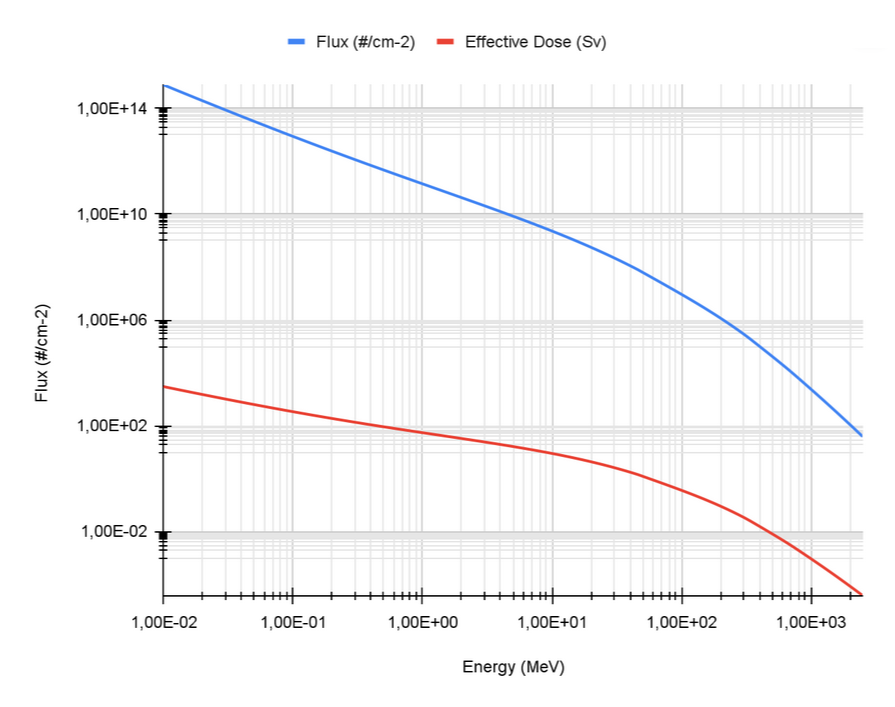
\includegraphics[width=.8\textwidth]{img/ED 1989.png}
\caption{SEP protons flux (count/cm-2) per energy and absorbed dose for a 70 Kg person during the whole duration of the 1989 solar event.}
\end{figure}

\subsection{Shielding}


Shadow shielding is a concept discussed in \citet{mclaren2010} as well as in \citet{hoffman1997}, it consist of using the NTR internal shield to block the line of sight from the reactor. The LN2 tank can also be placed between crew quarters and the reactor to protect the astronauts from the build up of radiations during the burn.\\

\citet{hoffman1997} proposes the use of aluminum shields as a radiation mitigation method, newer technologies such as Metal Hydrides Multi-Layered Radiation Shields as exposed in \citet{sreedevi2025effectiveness} could allow to make the different shielding lighter as Lithium Hydride has a density of 0.82 g.cm-3 compared to Aluminum's 2.7 g/cm-3 and is close to 2.3 time more absorbent for the same thickness. \\
\begin{figure}[hbtp]
\centering
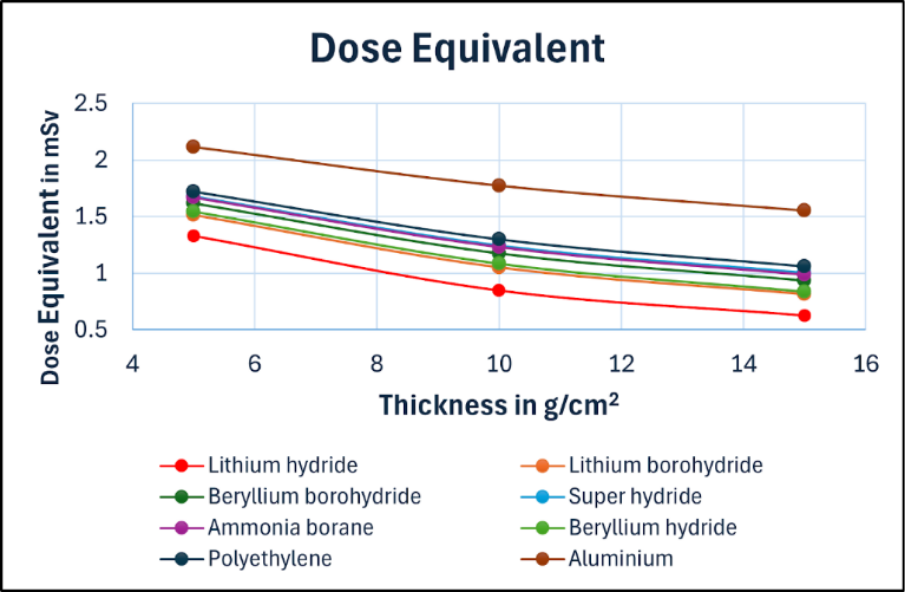
\includegraphics[width=.75\textwidth]{img/dose lih.png}
\caption{figure}{Variation of dose equivalent with thickness of various hydrides, polyethylene and aluminum, simulated by HZETRN}
\end{figure}



A shield weight of 0.9 tonnes is put forward in \citet{hoffman1997}, that weight could be decreased by 2.3 by using Lithium Hydride bringing it down to 0.4 tonnes.\\
It is also worth mentioning that only crewed mission need such shielding. \citet{hoffman1997} highlights a four launch plan for the exploration of Mars. Only one of those would carry humans.

Figure 4.5 shows the CSDA range for both aluminum and hydrogen as computed by the PSTAR algorithm, lithium hydride could not be computed as it is not in that database but it can be inferred that it would be 2.3 times smaller than Al.

\newpage



\chapter{Discussion}
% 	considers whether the data you obtained support the hypothesis 	explores the implications of your finding and judges the potential limitations of your experimental design
\quad This report shows that nuclear propulsion is a very promising technology that could heavily reduce the weight of rockets sent from the surface to space. Something that can't be ignored as the cost to send payload into orbit grown exponentially with its weight.\\

Even if this technologies is heartening one must not forget that strapping a nuclear reactor so close to people has some health risks, and therefore heavy shielding is needed.
This drawback would still yield lighter rockets as has been shown in 2.1.1 were NTRs lighter nature was affirmed and in 2.2.2 where a study showed that lighter than aluminum shields could be used thus making the rocket even lighter\\

On top of that must added that has was shown in 1.2 space is a very hostile environment radiation wise. People must therefore be shielded of radiations anyways.\\

A point must as well be made for space weather prediction, as solar event are yet to be foretasted with great advance, as of today forecast models only give a 2 to 3 day head's up until we are hit by solar storms. For the duration of the missions studied in this report such delays are unacceptable and mitigation strategies must be put in place.\\
\citet{valinia2022safe} highlights different recommendations for different events such as confinement on the surface if certain level of radiation are observed or foretasted. As for free space, eg. transit, the crew would take shelter in some heavier shielded part of the capsule.\\
\newpage
With sufficient shielding, crews could be as close as reasonably possible to the IAEA guideline for occupational workers. It would seem useful to note that the limits put forth by the IAEA are prone to change and might need to be adjusted for space workers as a new category of occupational workers. NASA uses a "dose over career" thinking for their radiation exposure mitigation, following the "as low as reasonably possible" philosophy.\\

Assuming our Muskian point of view the point could be made that although the crew would be exposed to a higher than legislated amount of radiation this journey would be one of the "once in a lifetime" event and that the scientific / cultural / political / ... gains would outweigh the risks the crew would be taking. It is worth mentioning that a lot of the risks of space missions where not discussed in this work.\\
As can be observed in 4.6 the TIPS procedure can expose a patient to a dose as big as 1.4 Sv in the span of 60-90 minutes. And has a 75\% survival rate after 5 years (mostly due to comorbidities as it is an emergency procedure).\\

A last point for nuclear propulsion is that though other high $I_{sp}$, nuclear free technologies exist, such as ionic propulsion or solar sails, they are for from functional yet and require high amount of solar energy to work which is a problem as soon as you leave the inner solar system as the solar iradiance weakens rapidly due to the inverse square law making such solutions, ironically, unconceivable without nuclear energy production.\\

During the debate it was brought up that the environmental effect of a failure at launch of the reactor would yield catastrophic environmental effect such as what happened in the Cosmos 954 incident over Canada that contaminated a surface of roughly 100000 square km where the amount of airborne uranium, in the most affected area, nearly doubled.\\

Such risks must be taken into account, such as designing the reactor so it can't reach critical mass with reentry or with an explosion of the orbital rocket.\\

The question of the recycling of the nuclear fissile material and byproduct wasn't addressed in the report as it is quite a complicated subject still prone to debate today. Some put forward burial solutions and others advocate for ditching the reactors in Earth or even Solar orbit.\\



\chapter{Conclusion}

\quad This report brought forward elements to answer weather nuclear energy was a technological prerequisite or a danger for the environment.\\
This question, far from trivial needs to be explored further than it has been here before a final answer can be given with any certainty, tough, with what we have learned we can try to bring some element into the reflection.\\

This report showed the use of NTRs in making the journey from Earth to Mars possible as well as some of the radioactive risks and mitigation that would be involved in such a mission.\\

On the subject of GCRs and SEP, proper shielding could be manufactured with today's technology and could therefore keep the crew safe. The radiations from the core could be managed in much the same way.\\

For all these reasons this report advocates that Nuclear Energy, though it is dangerous as it may be in its densely energetic nature doesn't have to be gamble with and would actually constitute a set of necessary tools for space exploration whilst we keep developing newer, greener, more efficient technologies to one day replace them effectively.

\chapter*{Acronyms}

\textbf{GCR: } Galactic Cosmic Ray\\
\textbf{SEP: } Solar Event Particles\\
\textbf{CEO: } Chief Executive Officer\\
\textbf{NTR: } Nuclear Thermal Rocket\\

\newpage


\bibliography{references}

\chapter{Appendix}

\begin{figure}[hbtp]
\centering
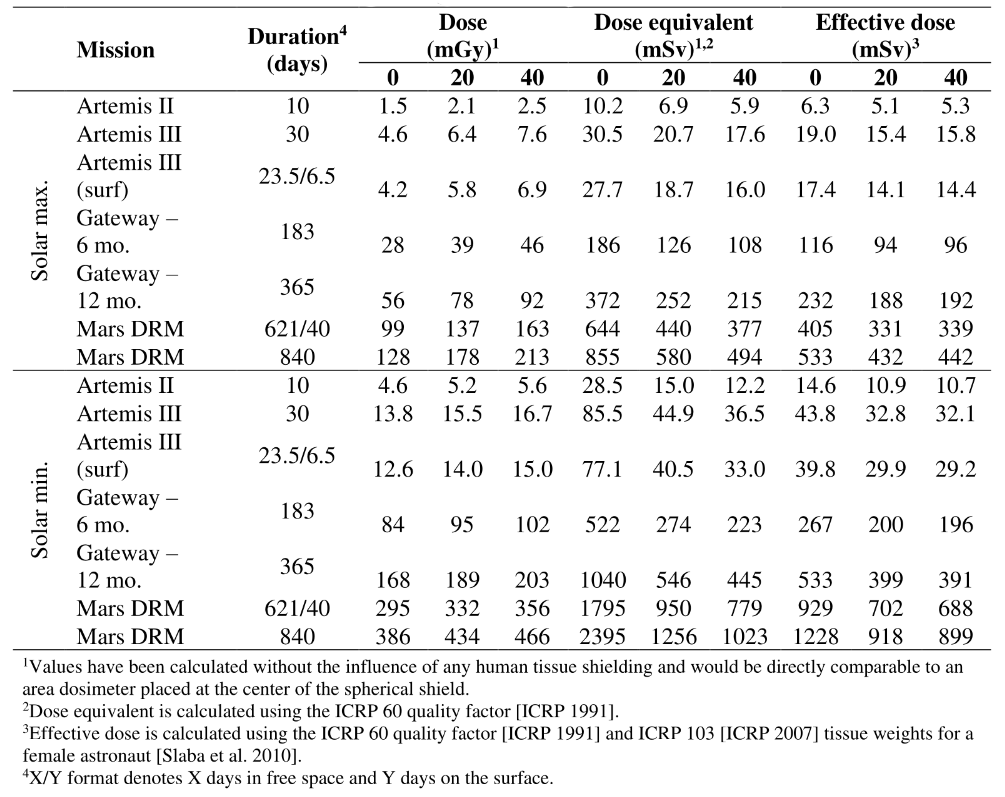
\includegraphics[width=1\textwidth]{img/extrapo.png}
\caption{Mission exposures derived by scaling daily values from Figure 4.2 by corresponding mission segment duration, from \citet{hoffman1997}}
\end{figure}

\begin{figure}[hbtp]
\centering
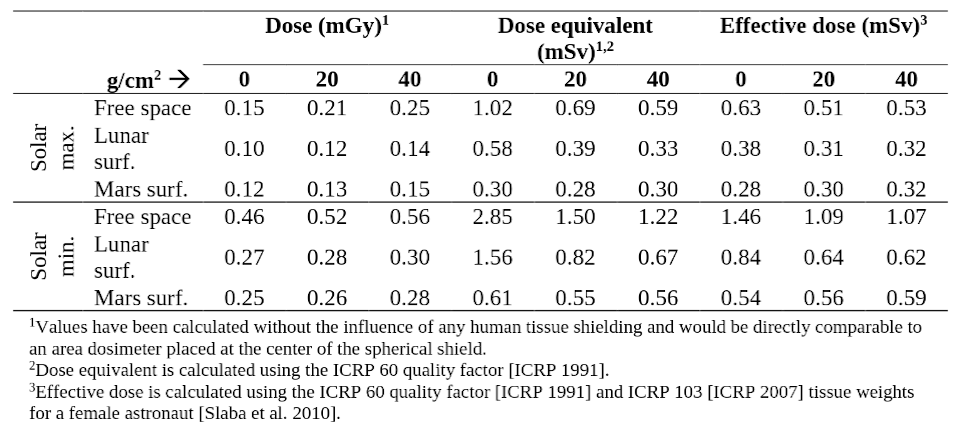
\includegraphics[width=1\textwidth]{img/data.png}
\caption{Daily exposure within 0, 20, and 40 g/cm2 spherical aluminum shielding in free space and on surface of Moon and Mars for solar minimum (2009) and solar maximum (2001) GCR conditions, from \citet{hoffman1997}}
\end{figure}

\begin{figure}[hbtp]
\centering
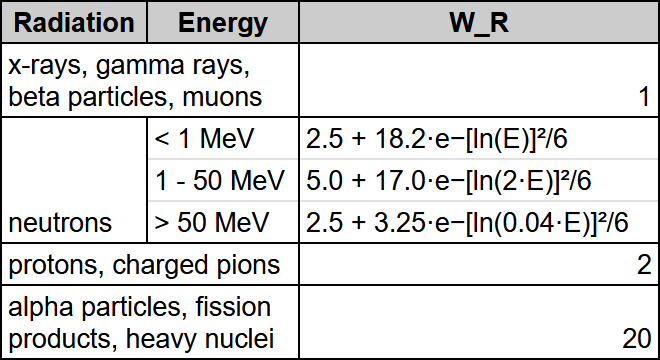
\includegraphics[width=1\textwidth]{img/Wr.png}
\caption{Radiation weighting factors $W_R$ used to represent relative biological effectiveness according to ICRP report \citet{valentin20072007}}
\end{figure}

\begin{figure}[hbtp]
\centering
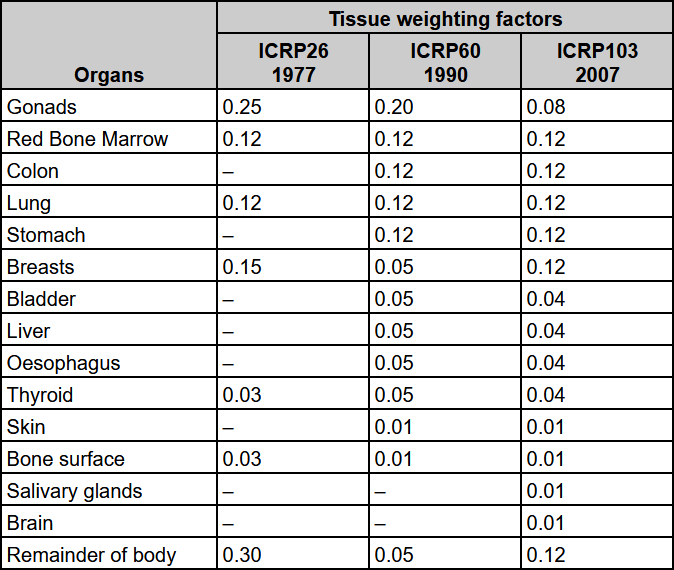
\includegraphics[width=1\textwidth]{img/Wh.png}
\caption{Weighting factors ($W_H$) for different tissues}
\end{figure}

\begin{figure}[hbtp]
\centering
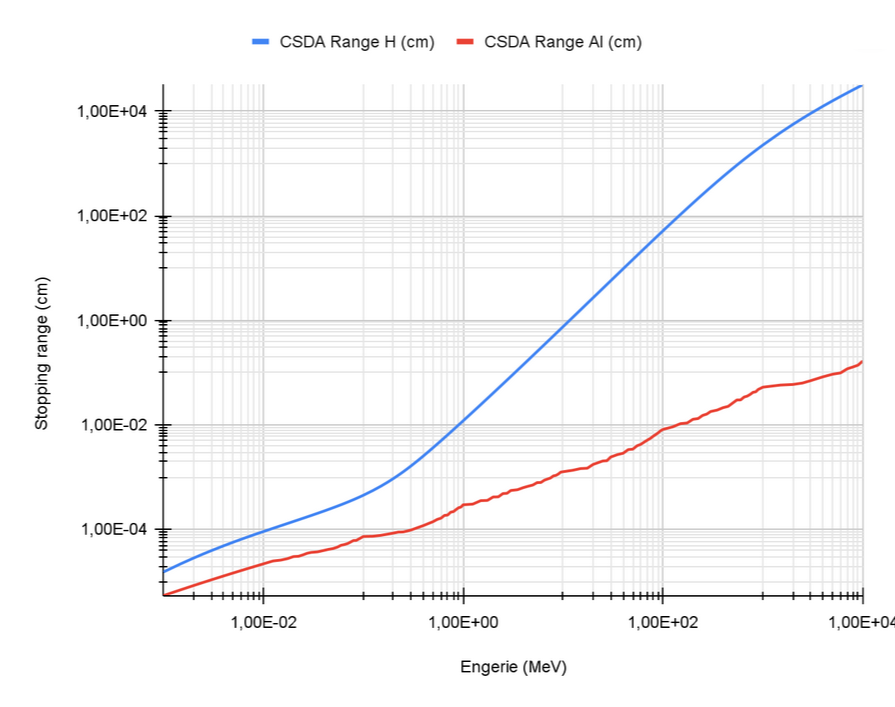
\includegraphics[width=1\textwidth]{img/ranges.png}
\caption{Stoping distance (cm) for protons of different energy levels (MeV) for hydrogen and aluminum}
\end{figure}

\begin{figure}[hbtp]
\centering
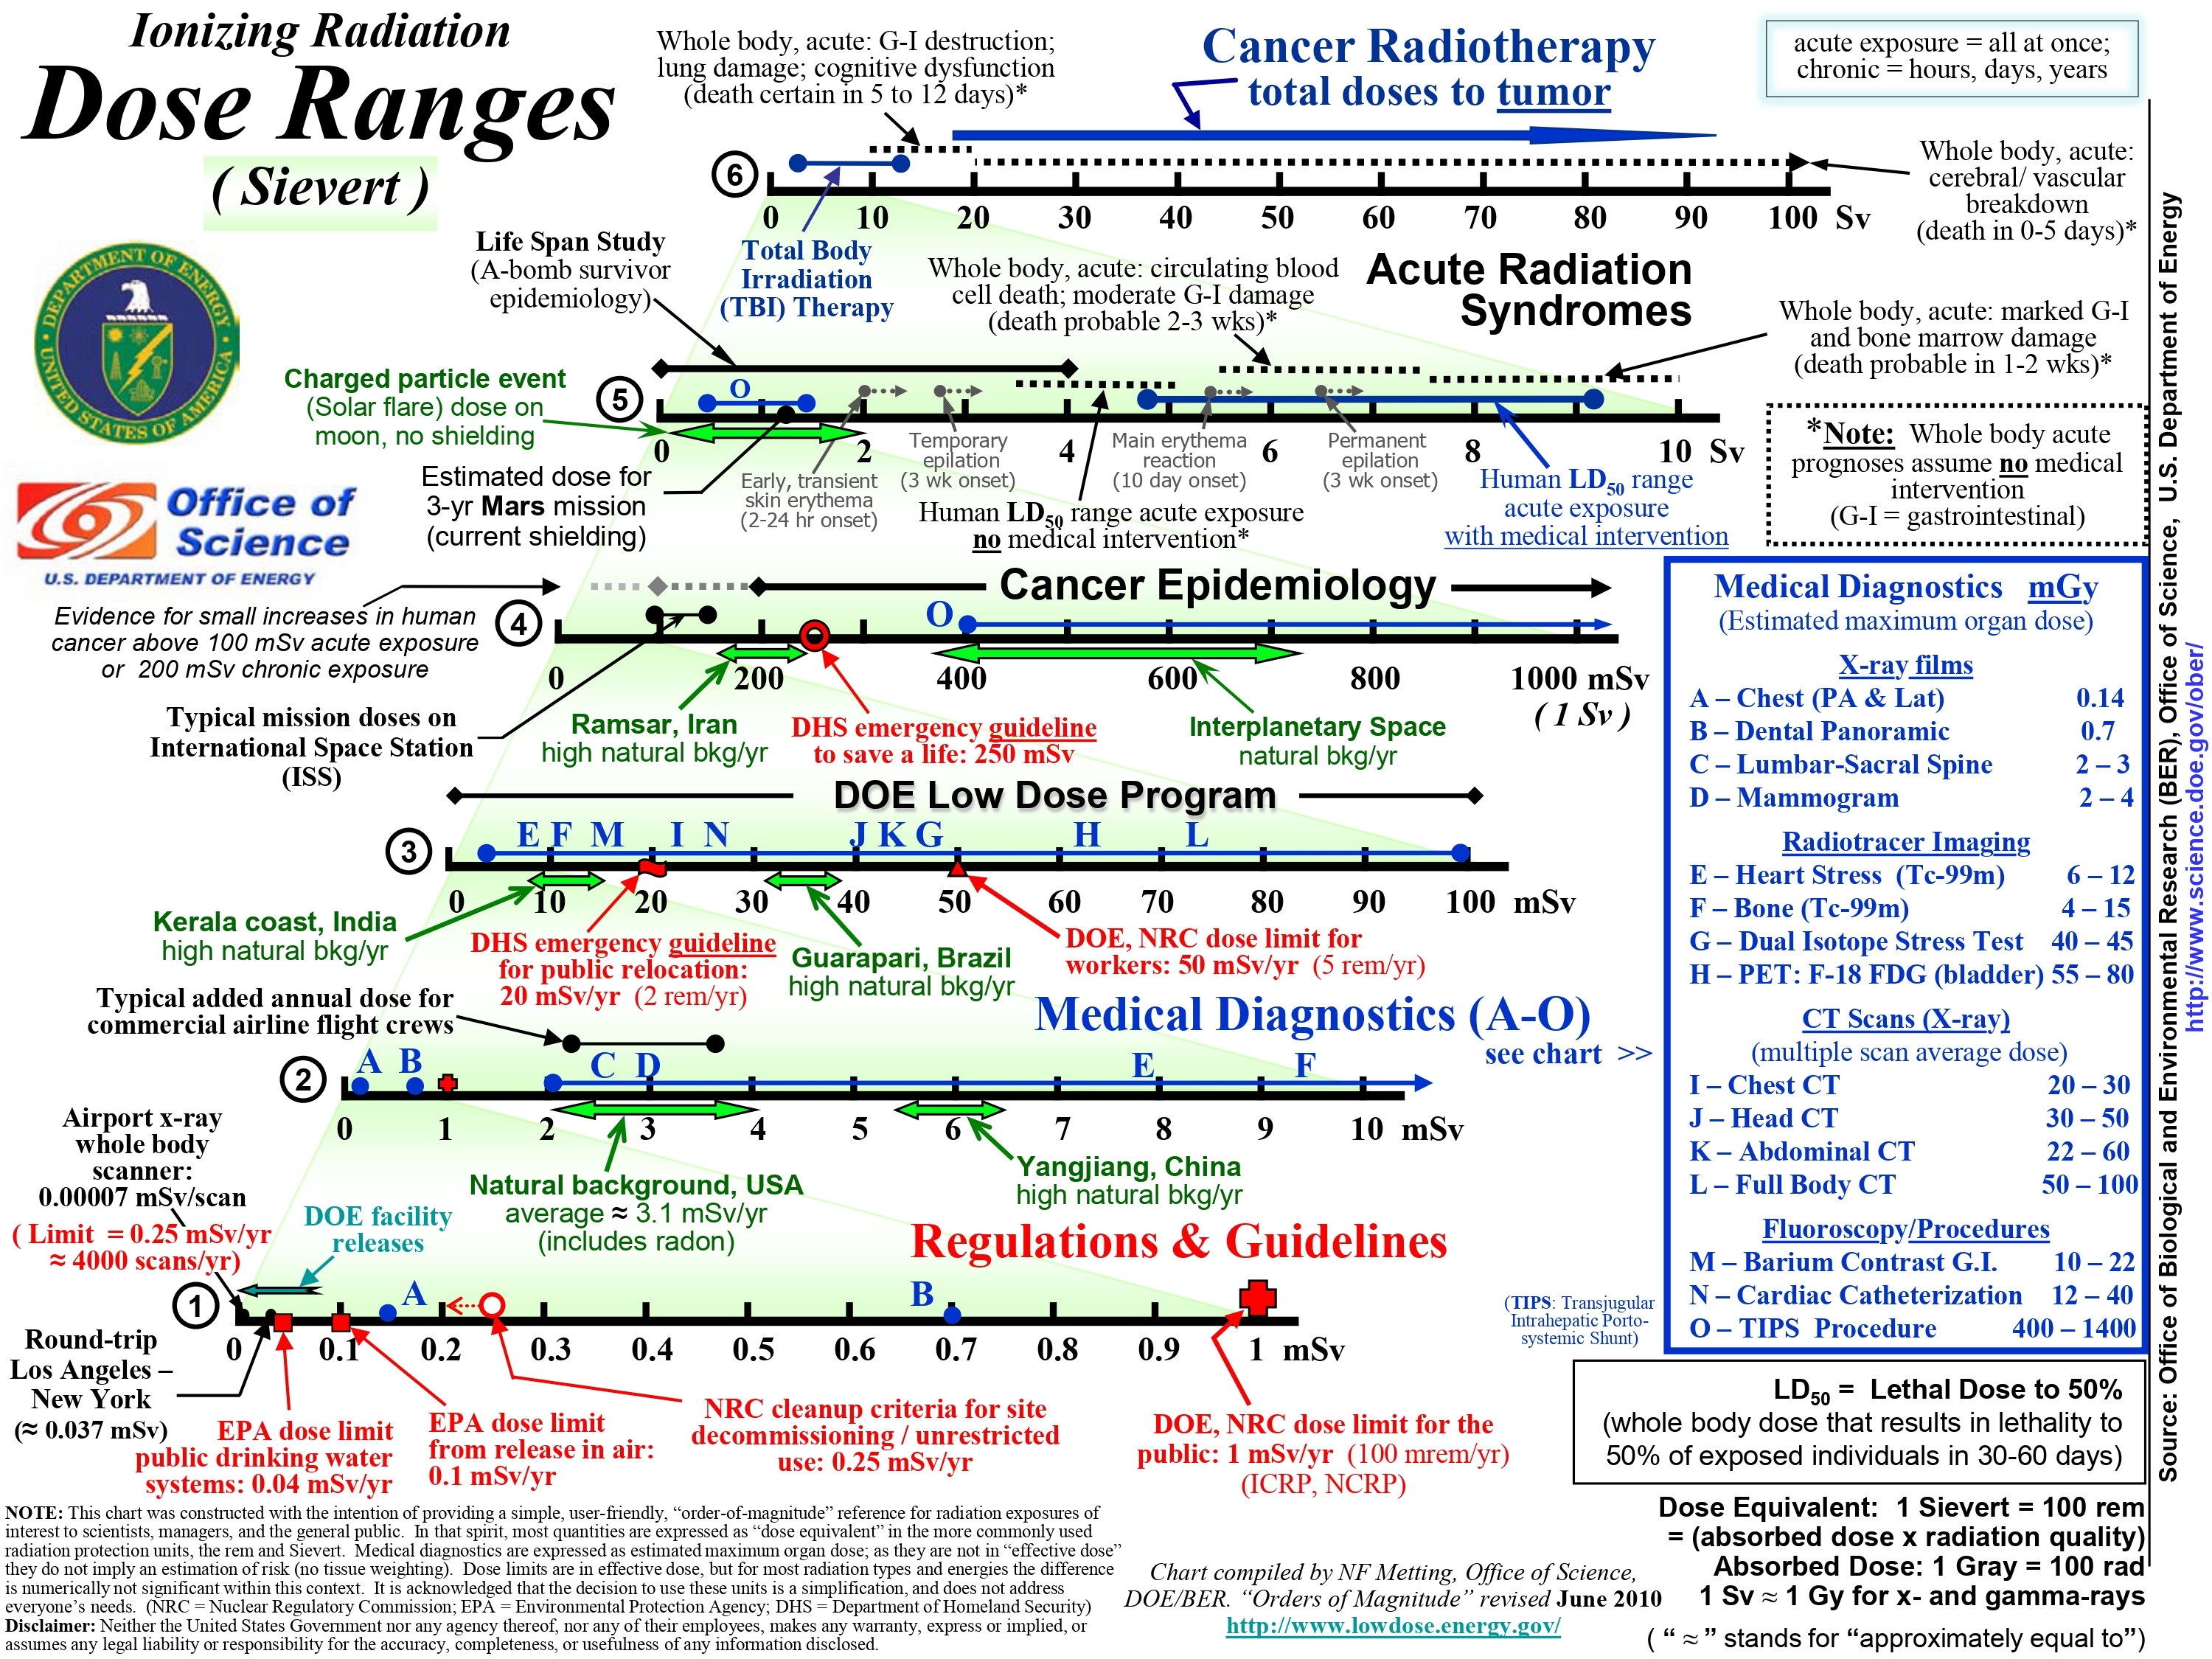
\includegraphics[width=1\textwidth]{img/ML120970113_pages-to-jpg-0002.jpg}
\caption{Dose range and their health effects, USA's department of energy}
\end{figure}

\begin{figure}[hbtp]
\centering
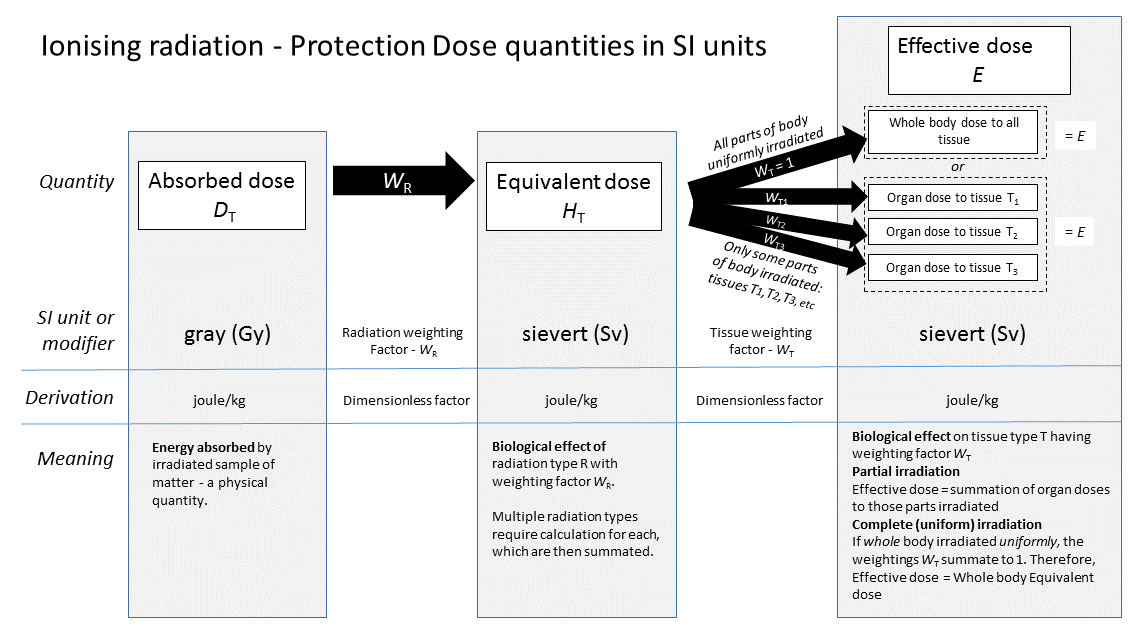
\includegraphics[width=1\textwidth]{img/SI_Radiation_dose_units.png}
\caption{Graphic showing relationships of protection dose quantities in SI units\\
 Doug Sim - Own work}
\end{figure}


\end{document}